\chapter{
ساخت مدار با
Logisim
}
\section{جمع‌کننده کامل}
\subsection*{تئوری آزمایش}
Full Adder
یک مدار ترکیبی دیجیتال است که سه ورودی گرفته و دو خروجی می‌دهد.
یکی از این سه ورودی ره به عنوان کری ورودی می‌شناسیم و دو تای دیگر متغییرهایی هستند که قرار است جمع شوند.
خروجی این مدار نیز یکی بیت جمع و دیگر بیت کری خروجی است.

\begin{figure}[h]
\centering
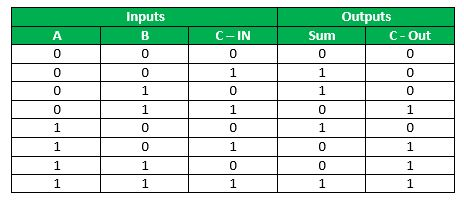
\includegraphics[scale=1]{Experimental Methods/table.jpg}
\caption{جدول صحت
یک جمع کننده کامل
}
\end{figure}

مطابق این جدول برای بیت‌های خروجی یک مدار بدست می‌آید که آن را در نرم‌افزار رسم کرده و شبیه‌سازی می‌کنیم.

\subsection{شرح آزمایش}
\begin{figure}[h]
\centering
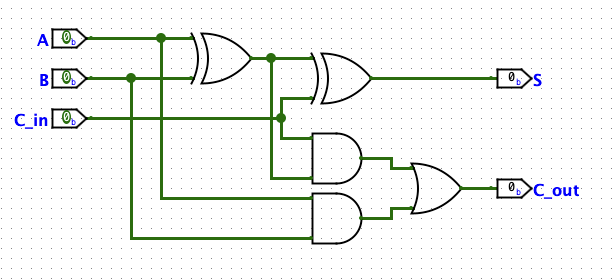
\includegraphics[scale=0.6]{Experimental Methods/1.png}
\caption{
مدار جمع‌کننده کامل در نرم‌افزار
Logisim
}
\end{figure}

ورودی‌ها و خروجی‌ها را به تعداد مناسب قرار داده و برای آن‌ها لیبل مناسب می‌زنیم.

حال گیت‌ها را قرار داده و اتصالات را برقرار می‌کنیم.

در نهایت با استفاده از ابزار
«دست»
که از منوی بالای صفحه قابل انتخاب است ورودی‌های مدار را تغییر می‌دهیم و تاثیر آن را در خروجی‌ها می‌بینیم.


\section{
جمع‌کننده/تفریق‌کننده
4 بیتی
}
برای کم کردن
B
از
A
کافی است هر دو عدد را در مکمل دو ببریم و سپس با جمع کننده‌ی عادی آن‌ها را جمع بزنیم.
حاصل نیز در مکمل دو خواهد بود.

همچنین می‌دانیم برای پیدا کردن مکمل دوی یک عدد باید بیت‌های آن را معکوس کرده سپس عدد نهایی را با یک جمع کنیم.
برای معکوس کردن بیت‌ها کافی است آن‌ها را با ورودی‌ای که اگر یک شود این اتفاق بیفتد
XOR کنیم.
که اگر این ورودی کنترلی یک باشد خروجی معکوس بیت‌ها و در غیر این صورت خود آن‌ها خواهد بود.

حالا این ورودی‌های معکوس شده‌ی مشروط را با هم جمع می‌کنیم. آن یکی هم که باید جمع می‌کردیم را در کری ورودی جمع‌کننده‌ی ابتدایی قرار می‌دهیم. نتیجه‌ی نهایی در شکل آمده است.

\begin{figure}[h]
\centering
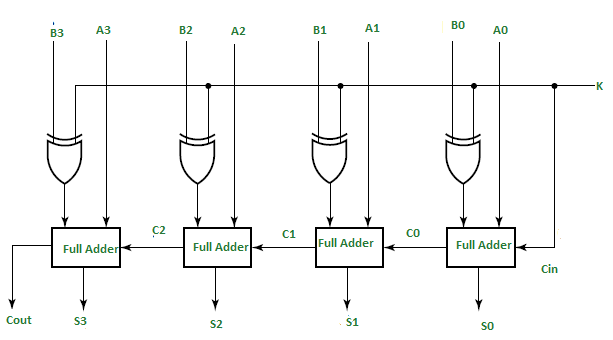
\includegraphics[scale=1]{Experimental Methods/2.png}
\caption{
شماتیک مدار جمع‌کننده/تفریق‌کننده کنترلی
}
\end{figure}

\subsection*{شرح آزمایش}
مطابق شکل نشان‌داده شده و مطابق مدار جمع کننده‌ی کامل که در بخش قبل بستیم مدار نهایی را می‌بندیم.

در انتها می‌توانیم کمی با آن بازی کنیم و آن را برای حالات مختلف تست کنیم.

\begin{figure}[h]
\centering
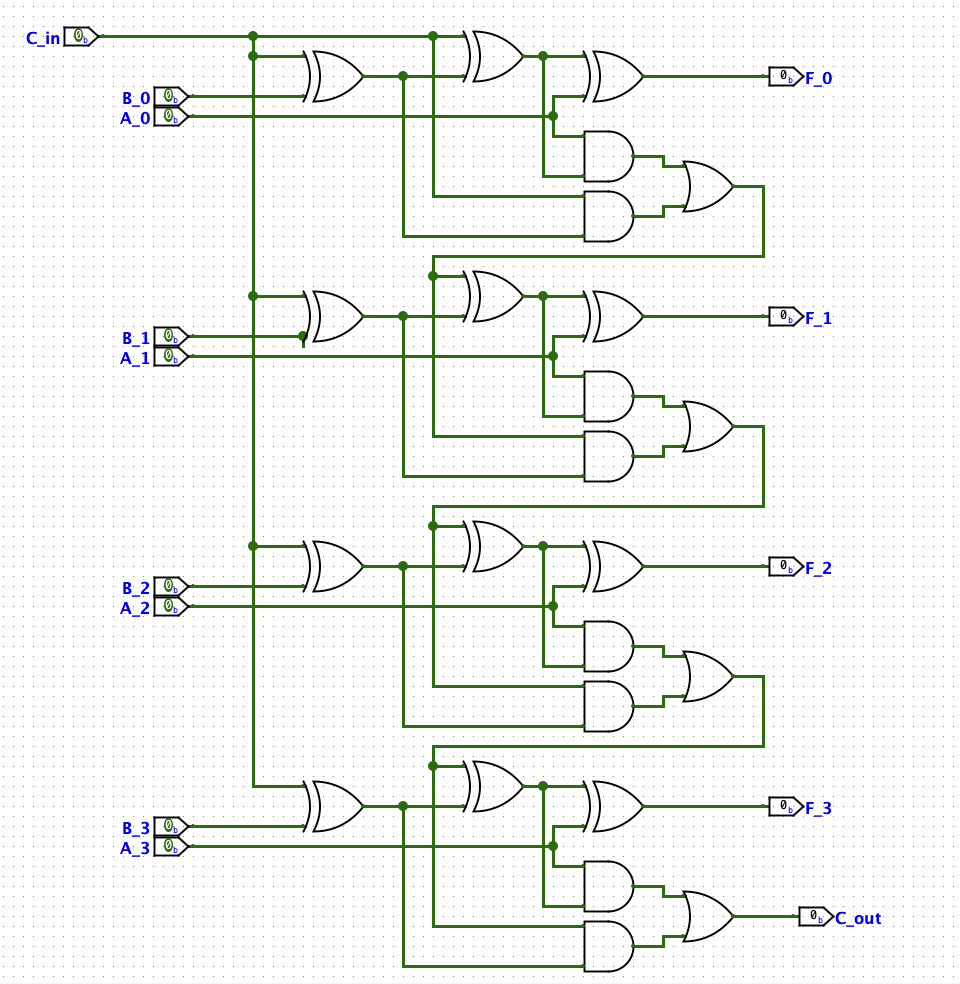
\includegraphics[scale=0.3]{Experimental Methods/3.png}
\caption{
مدار نهایی
}
\end{figure}